% ============================================================
% SECTION 3: KHẢO SÁT DỮ LIỆU NGUỒN
% ============================================================
\section{Khảo sát dữ liệu nguồn}

% --- Slide: Nguồn dữ liệu ---
\begin{frame}{Nguồn dữ liệu đầu vào}
\begin{itemize}
  \item \textbf{Nguồn chính:} bộ dữ liệu US Flight Delays 2015 (Kaggle/BTS).
  \item \textbf{4 tệp sử dụng trong ETL:}
\end{itemize}

\vspace{1mm}
\small\slideTablePad
\begin{table}
\centering
\begin{tabular}{|l|l|p{6.5cm}|}
\hline
\textbf{Tệp} & \textbf{Số lượng} & \textbf{Vai trò} \\
\hline
\texttt{flights.csv} & 5.819.079 dòng & Bảng giao dịch chính: lịch bay, thời gian thực tế, delay, hủy chuyến \\
\hline
\texttt{airlines.csv} & 14 hãng & Tra cứu mã IATA $\rightarrow$ tên hãng \\
\hline
\texttt{airports.csv} & 322 sân bay & Tra cứu tên sân bay, bang, tọa độ địa lý \\
\hline
\texttt{L\_AIRPORT\_ID.xls} & 6414 dòng & Quy đổi Airport ID dạng số về mã sân bay phục vụ join \\
\hline
\end{tabular}
\end{table}

\vspace{1mm}
\footnotesize
\textit{Mục tiêu khảo sát:} đánh giá chất lượng dữ liệu trước ETL để xác định quy tắc làm sạch có căn cứ.
\end{frame}

\begin{frame}{Nguồn dữ liệu đầu vào}
  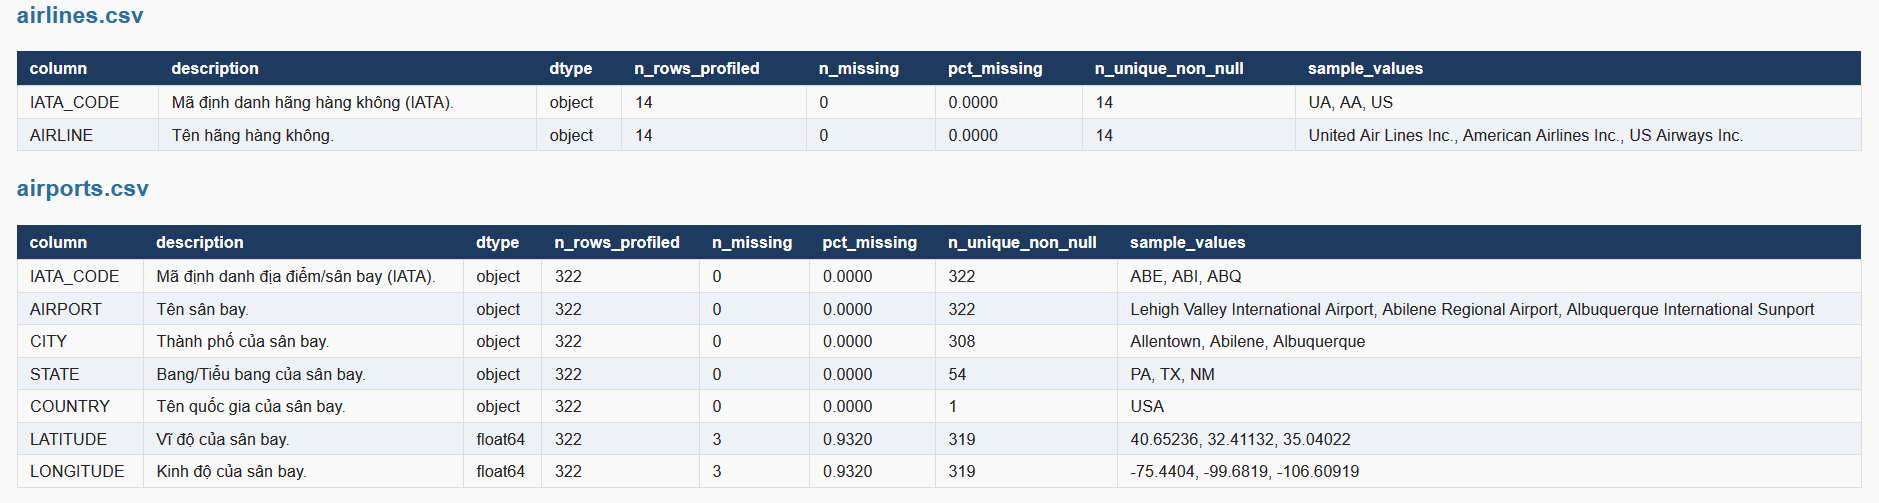
\includegraphics[width=\linewidth,height=0.72\textheight,keepaspectratio]{./images/eda/column_1.png}
\end{frame}

\begin{frame}{Nguồn dữ liệu đầu vào}
  \centering
  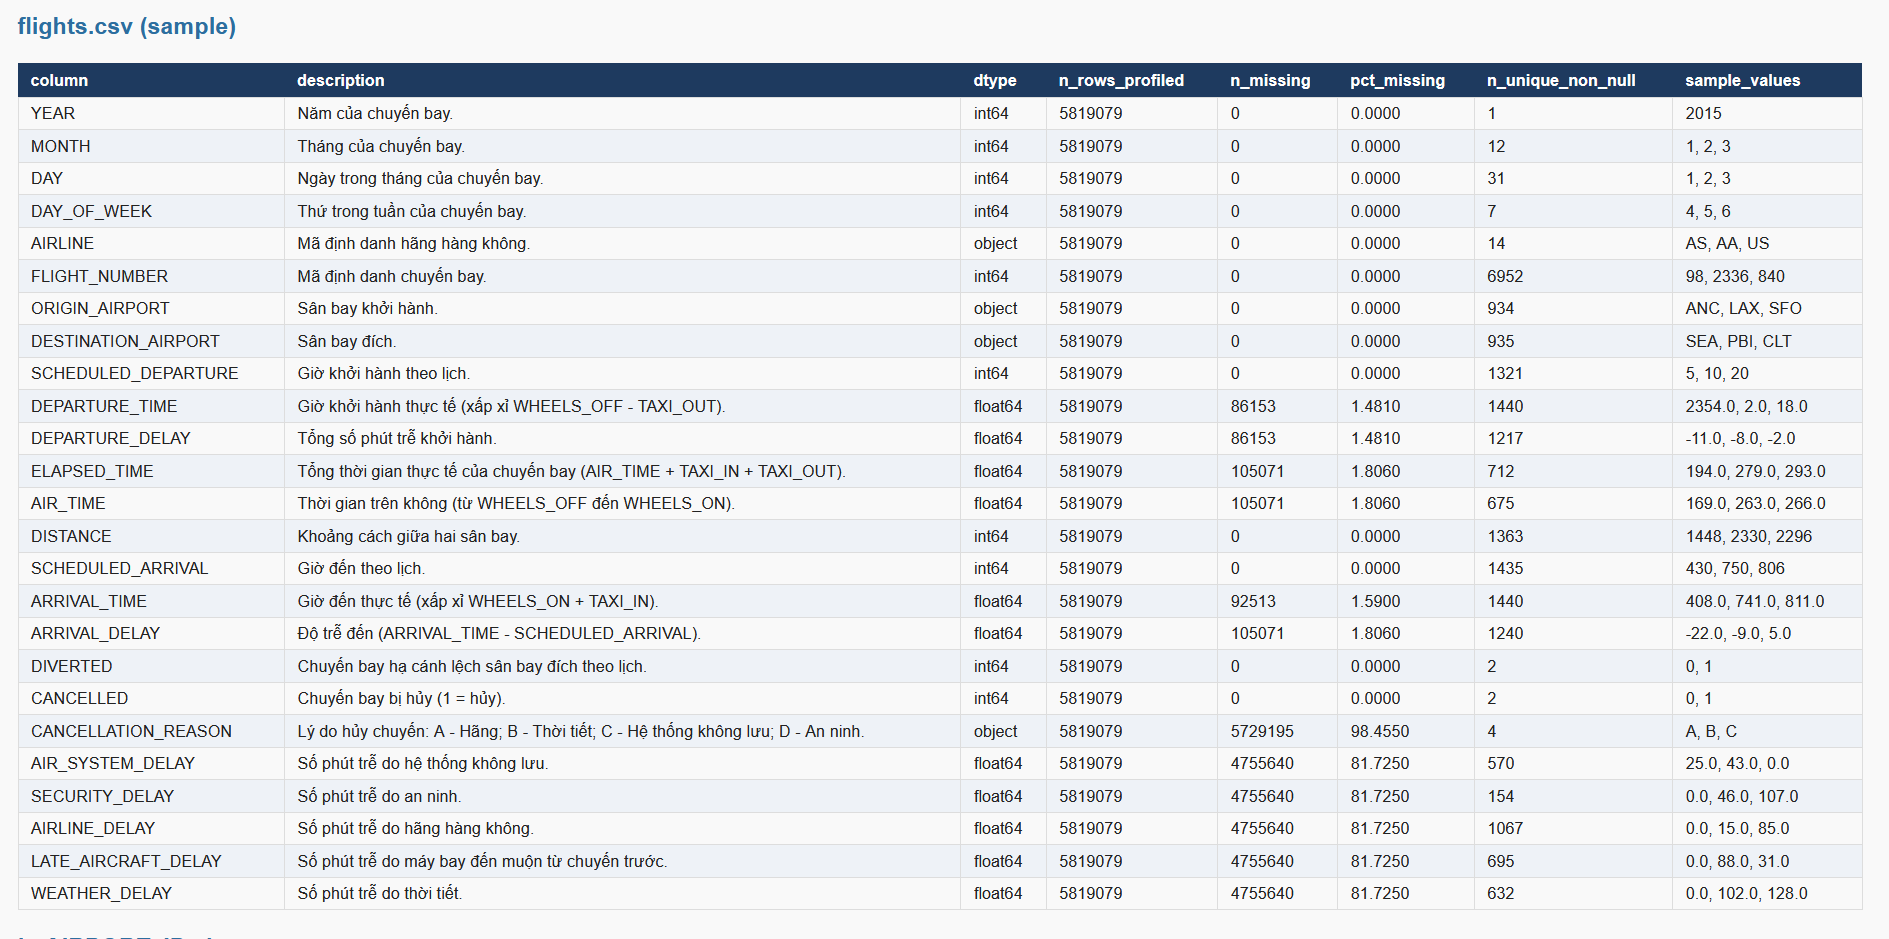
\includegraphics[width=\linewidth,height=0.72\textheight,keepaspectratio]{./images/eda/column_2.png}
\end{frame}

% --- Slide: Missing/Outlier ---
\begin{frame}{Tỷ lệ missing ở các cột}
  \begin{center}
    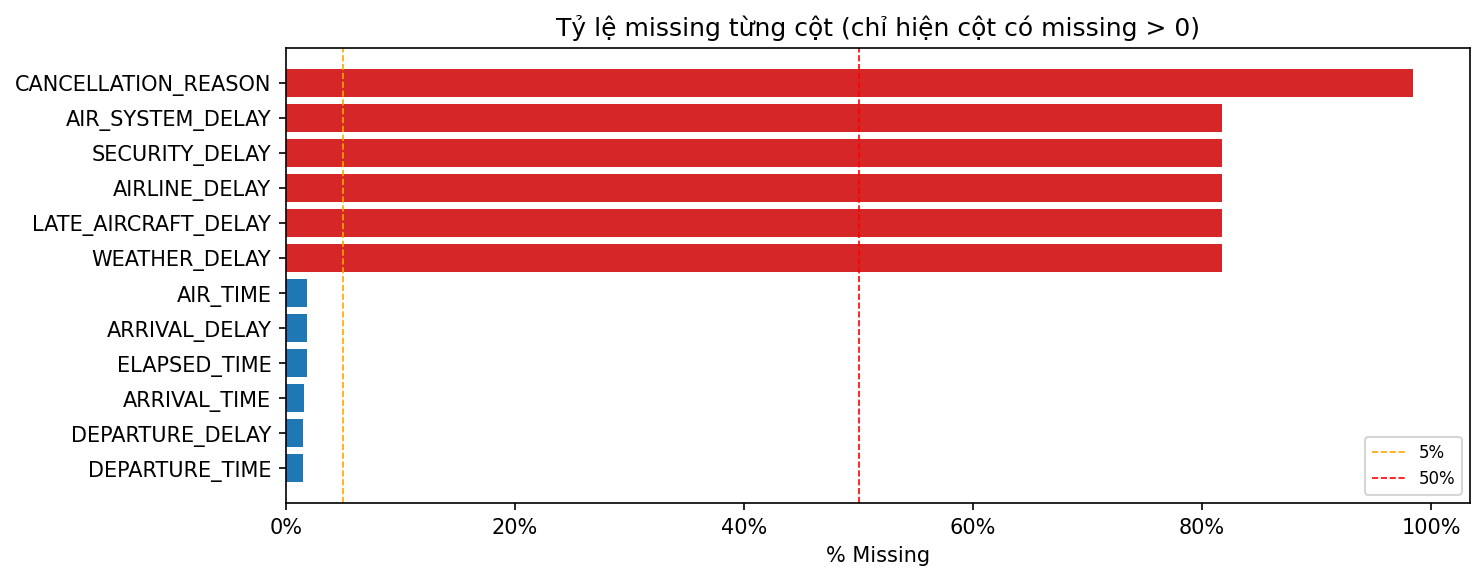
\includegraphics[width=\linewidth,height=0.5\textheight,keepaspectratio]{./images/eda/eda_missing_bar.png}
  \end{center}
  \begin{small}
  \textbf{Phát hiện chính trên \texttt{flights.csv}:}
  \begin{itemize}
    \item Nhóm delay thành phần (\texttt{AIR\_SYSTEM\_DELAY}, \texttt{AIRLINE\_DELAY}, \texttt{WEATHER\_DELAY}, \texttt{LATE\_AIRCRAFT\_DELAY}, \texttt{SECURITY\_DELAY}) thiếu khoảng \textbf{81.72\%}.
    \item Một số cột thời gian thực tế thiếu do chuyến hủy/chưa hoàn tất.
    \item Đề tài hướng đến xu hướng chậm chuyến nên không cần quan tâm đến tỷ lệ lớn \texttt{CANCELLATION\_REASON} bị missing.
  \end{itemize}
  \end{small}
\end{frame}

\begin{frame}{Kiểm tra chuyến đúng giờ}
  \begin{center}
    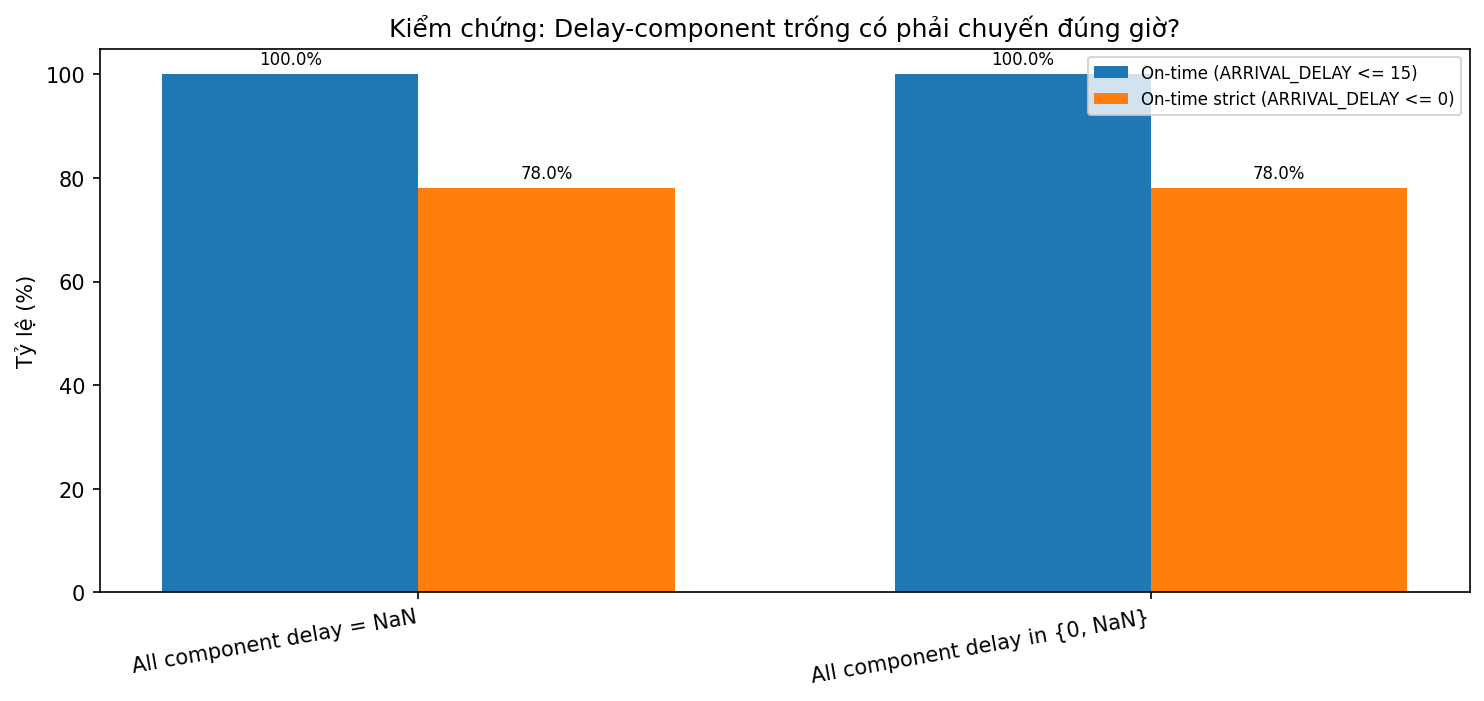
\includegraphics[width=\linewidth,height=0.5\textheight,keepaspectratio]{./images/eda/eda_delay_null_vs_ontime.png}
  \end{center}
  
  \begin{small}
  Ý nghĩa các giá trị 0 hoặc NaN được điền vào các cột delay thành phần:
  \begin{itemize}
    \item Với ngưỡng trễ $\leq$ 0 phút, 78 \% chuyến bay được coi là đúng giờ, nếu mở rộng ngưỡng xét tới 15 phút, tỷ lệ đạt 100\%.
    \item Chuyến bay được coi là đúng giờ với nhãn mục tiêu \texttt{is\_delayed\_15} = 0 nếu missing tất cả cột delay thành phần (NaN hoặc 0) hoặc \texttt{CANCELLED} = 1 hoặc \texttt{DIVERTED} = 1, = 1 nếu \texttt{ARRIVAL\_DELAY} $\geq$ 15 phút.
  \end{itemize}
  \end{small}
\end{frame}

\begin{frame}{Phân phối delay}
  \begin{center}
    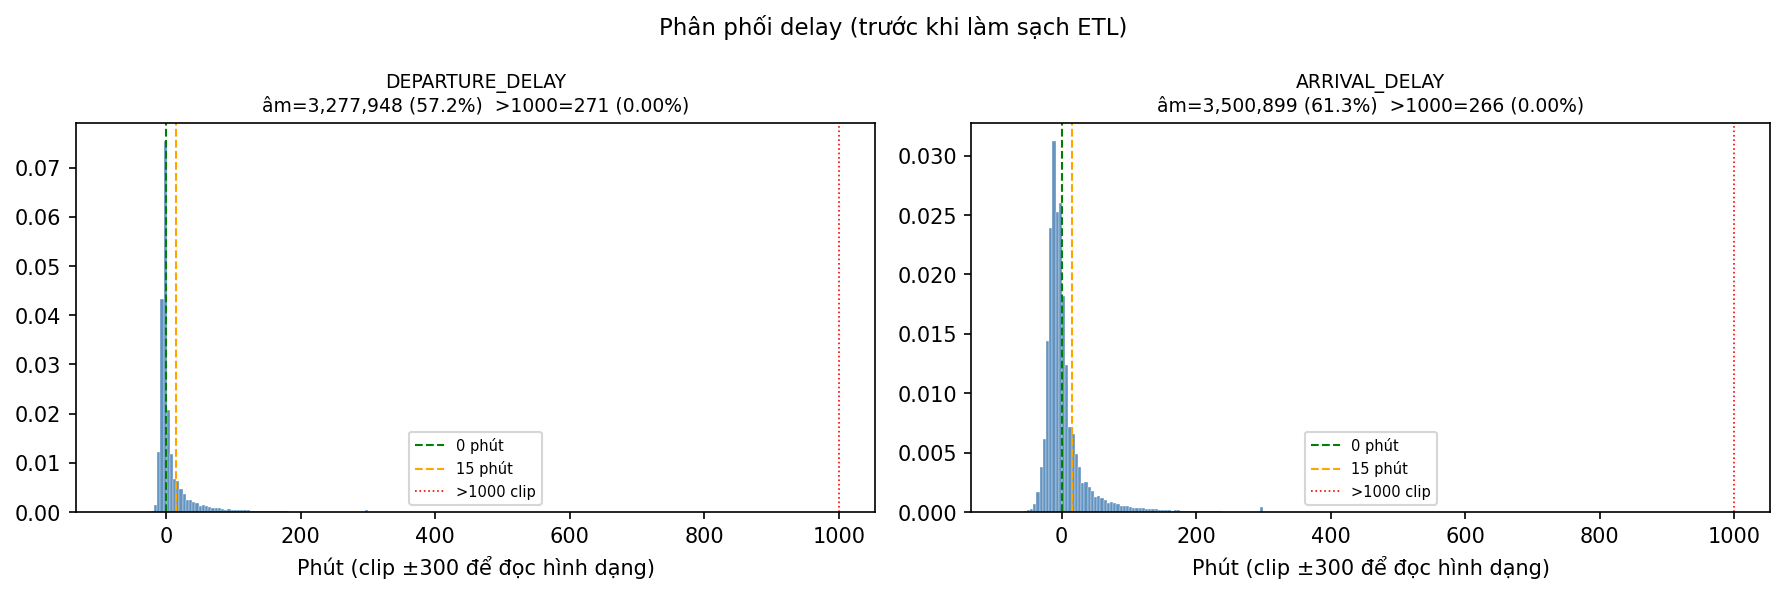
\includegraphics[width=\linewidth,height=0.5\textheight,keepaspectratio]{./images/eda/eda_delay_dist.png}
  \end{center}
  
  \begin{small}
  Phân phối \texttt{DEPARTURE\_DELAY} và \texttt{ARRIVAL\_DELAY} trên toàn bộ dữ liệu:
  \begin{itemize}
    \item Delay âm = chuyến đến sớm hơn lịch (bình thường). $\rightarrow$ \textit{giữ nguyên}.
    \item Delay >1000 phút = hoãn qua ngày (hiếm nhưng thật). $\rightarrow$ \textit{giữ nguyên}. 
  \end{itemize}
  \end{small}
\end{frame}

\begin{frame}{Phân phối quãng đường và thời gian bay}
  \begin{center}
    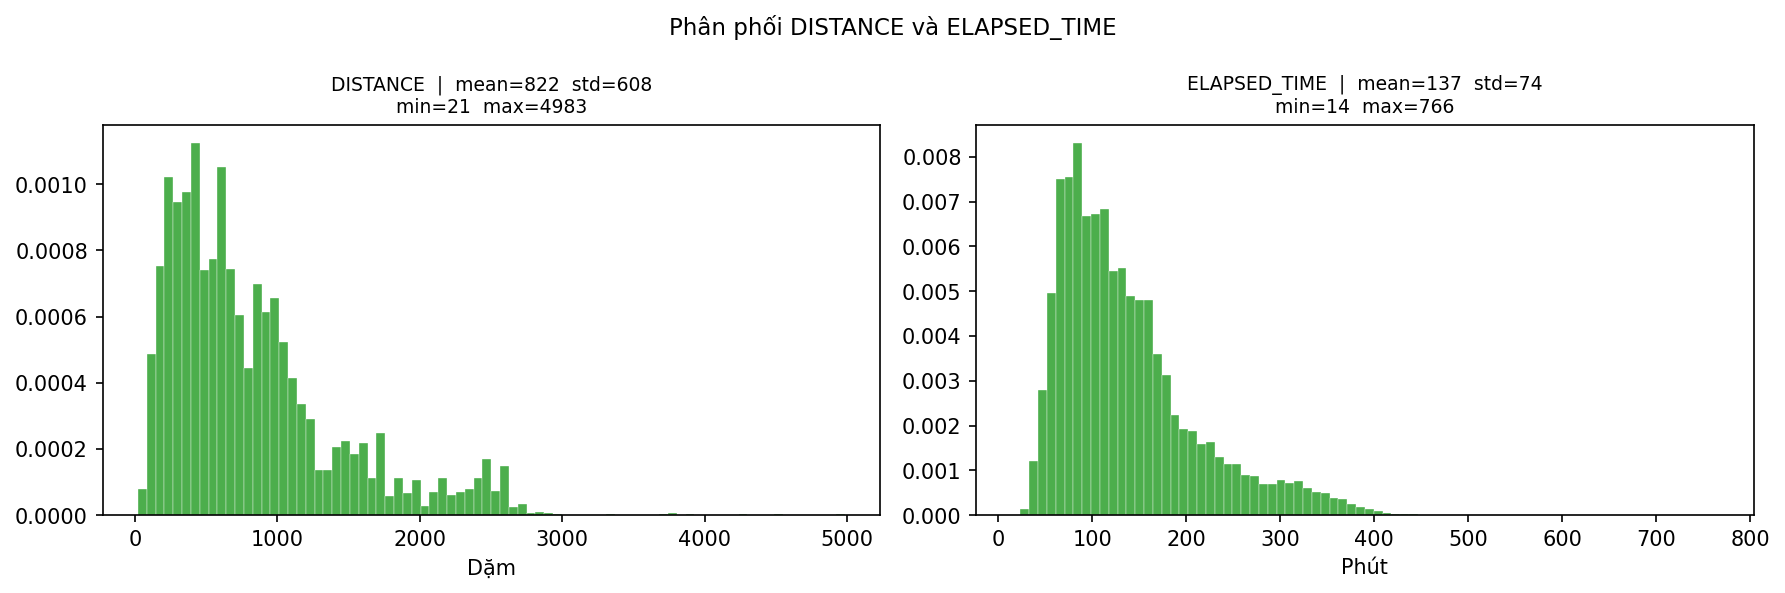
\includegraphics[width=\linewidth,height=0.45\textheight,keepaspectratio]{./images/eda/eda_distance_dist.png}
  \end{center}
  
  \begin{small}
  Phân phối \texttt{DISTANCE} và \texttt{ELAPSED\_TIME} trên toàn bộ dữ liệu:
  \begin{itemize}
    \item \textbf{DISTANCE:} Tập trung chủ yếu 300--1500 dặm; đuôi kéo dài gần 5000 dặm.
    \item \textbf{ELAPSED\_TIME:} Tập trung quanh 80--200 phút; các giá trị >700 phút.
    \item \textbf{Đặc điểm:} Cả hai biến đều có phân phối lệch phải với nhiều giá trị ngoại lai (Outliers).
    \item \textbf{Xử lý missing:} điền Median, đảm bảo tính ổn định, không bị nhiễu bởi các chuyến bay dài.
  \end{itemize}
  \end{small}
\end{frame}

\begin{frame}{Tổng kết khảo sát dữ liệu nguồn}
  \textbf{Kết luận sau quá trình EDA:}
  \begin{itemize}
    \item \textbf{Quy mô dữ liệu:} Dữ liệu rất lớn ($\approx$ 5.8 triệu dòng), đủ độ tin cậy để huấn luyện các mô hình dự báo sâu.
    \item \textbf{Thách thức về chất lượng:} 
      \begin{itemize}
        \item Tỷ lệ missing tập trung ở nhóm nguyên nhân delay ($\approx$ 82\%) $\rightarrow$ Cần xử lý nhất quán giữa giá trị \texttt{NaN} và $0$.
        \item Dữ liệu bị nhiễu và lệch phải mạnh ở các biến thời gian và khoảng cách.
      \end{itemize}
    \item \textbf{Chiến lược xử lý (Tiền đề cho ETL):}
      \begin{itemize}
        \item Giữ lại các giá trị ngoại lai (outliers) cực đại vì đây là thực tế vận hành (delay kéo dài, bay đường dài).
        \item Ưu tiên sử dụng \textbf{Median} và \textbf{Mode} để điền khuyết nhằm bảo toàn đặc tính phân phối tự nhiên.
      \end{itemize}
    \item \textbf{Độ sẵn sàng:} Dữ liệu đã được định hình rõ các đặc trưng quan trọng (\texttt{elapsed\_time}, \texttt{distance}, \texttt{is\_delayed\_15}), sẵn sàng cho giai đoạn chuẩn hóa và xây dựng kho dữ liệu (Data Warehouse).
  \end{itemize}
\end{frame}